\chapter{String Theory and M-Theory}

We now turn from open strings to closed strings, but the lecture does not begin with the loop itself. It begins with a brief piece of mathematics that will later reappear in a rather beautiful way. The guiding idea is that a symmetry should have a generator, and that for the closed string the apparently innocent choice of where \(\sigma=0\) sits on the loop is not a physical choice at all. Once that point is taken seriously, the familiar Fourier analysis of the string, the doubled left- and right-moving oscillator structure, the level-matching rule, and finally the appearance of the graviton all fall into place.

\section{Noether's Theorem as a Prelude}

Before moving to closed strings, we remind ourselves of one formula and one way of thinking. We do not need a proof of Noether's theorem here; we only need the form of the conserved generator.

If the Lagrangian depends on coordinates \(q_i\) and their velocities \(\dot q_i\), then the canonical momentum is
\begin{equation}
p_i=\frac{\partial L}{\partial \dot q_i}.
\end{equation}
For an infinitesimal transformation \(q_i\to q_i+\delta q_i\), the corresponding Noether generator is, schematically,
\begin{equation}
Q_{\mathrm{Noether}}=\sum_i p_i\,\delta q_i.
\end{equation}
In quantum mechanics this becomes the operator that generates the small transformation on the wave function.

The lecture gives the elementary example of a small rotation in the \(xy\)-plane. In that case one may write
\begin{equation}
\delta x = y\,\epsilon,
\qquad
\delta y = -x\,\epsilon,
\end{equation}
with \(\epsilon\) a small angle. The conserved charge is then angular momentum. We do not pursue the example further, because the real point is simply this: later on, a shift of the \(\sigma\)-coordinate on a closed string will itself behave like a symmetry, and then the Noether point of view will become useful.

\section{Closed Strings, Marked Points, and Intrinsic Orientation}

A closed string is a string without endpoints. It is natural to parameterize it by
\begin{equation}
0\leq \sigma \leq 2\pi.
\end{equation}
One point on the loop is marked and called \(\sigma=0\), but nothing in the geometry suggests that this point is special. It is only a coordinate choice.

\begin{figure}[t]
\centering

\includegraphics[width=0.62\textwidth]{lecture_04_figure_02.png}
\caption{Closed string with a marked \(\sigma=0\) point.}
\end{figure}

It is useful to redraw the same idea cleanly. The loop is not meant to have any special shape; only the distinguished point matters.

\begin{figure}[t]
\centering
\begin{tikzpicture}[scale=1.1]
\draw
(0.2,1.0)
.. controls (1.2,1.6) and (2.5,1.4) .. (3.0,0.5)
.. controls (3.5,-0.5) and (2.7,-1.6) .. (1.8,-1.1)
.. controls (1.0,-1.8) and (-0.2,-1.4) .. (-0.4,-0.2)
.. controls (-0.6,0.6) and (-0.1,0.8) .. (0.2,1.0);
\fill (0.2,1.0) circle (1.5pt);
\node[above] at (0.2,1.05) {\(\sigma=0\)};
\draw[->] (4.0,-0.2) -- (5.0,-0.2);
\draw[->] (4.0,-0.2) -- (4.0,0.9);
\node[right] at (5.0,-0.2) {\(x\)};
\node[above] at (4.0,0.9) {\(y\)};
\end{tikzpicture}
\caption{A clean schematic of the same geometric setup.}
\end{figure}

The next point is subtle and must be made carefully. The orientation of the string is not its clockwise or counterclockwise placement in the \(xy\)-plane. One can lift the loop, turn it over, and put it back down. The orientation that matters is intrinsic: it is the direction in which \(\sigma\) increases. Thus a right-moving wave means a disturbance propagating toward larger \(\sigma\), and a left-moving wave means propagation toward smaller \(\sigma\). This distinction will matter all the way through the spectrum analysis.

\section{Periodic Boundary Conditions, Fourier Modes, and Energy Flow}

The coordinates of the closed string are the same kind of coordinates we already used for the open string, namely functions such as \(x(\sigma)\) and \(y(\sigma)\). The difference is that the boundary condition is now periodic:
\begin{equation}
x(0)=x(2\pi),
\qquad
y(0)=y(2\pi).
\end{equation}
That periodicity is the whole reason that exponentials \(e^{in\sigma}\) are the natural basis. The general Fourier expansion is
\begin{equation}
x(\sigma)=\sum_{n\in\mathbb Z} x_n e^{in\sigma},
\end{equation}
or, separating positive, negative, and zero modes,
\begin{equation}
x(\sigma)=x_0+\sum_{n>0}x_n e^{in\sigma}+\sum_{n>0}x_{-n}e^{-in\sigma},
\end{equation}
with an exactly analogous expansion for \(y(\sigma)\). The \(n=0\) term is the center of mass of the whole string. Positive and negative \(n\) label the two propagation directions along the string.

The lecture stresses that the frequency is proportional to \(|n|\), just as for the open string. So each mode is a harmonic oscillator, but now every frequency comes in two directional copies.

The Lagrangian has the same structure as before, except that the \(\sigma\)-integral now runs from \(0\) to \(2\pi\):
\begin{equation}
L \sim \int_0^{2\pi} d\sigma
\Big[
(\partial_\tau x)^2-(\partial_\sigma x)^2
+
(\partial_\tau y)^2-(\partial_\sigma y)^2
\Big].
\end{equation}
The corresponding energy has plus signs,
\begin{equation}
E \sim \int_0^{2\pi} d\sigma
\Big[
(\partial_\tau x)^2+(\partial_\sigma x)^2
+
(\partial_\tau y)^2+(\partial_\sigma y)^2
\Big].
\end{equation}
Now comes a very useful algebraic rearrangement. Susskind remarks that he is off by a factor of two on the board, so we write the standard corrected identity:
\begin{equation}
(\partial_\tau X)^2+(\partial_\sigma X)^2
=
\frac12\Big[
(\partial_\tau X+\partial_\sigma X)^2
+
(\partial_\tau X-\partial_\sigma X)^2
\Big].
\end{equation}
The same holds for \(Y\). This is the point where the energy splits into two independent pieces, one associated with one propagation direction and one associated with the other. For the closed string, left-moving and right-moving waves simply pass through one another.

It is worthwhile to keep a geometric picture of this in mind.

\begin{figure}[t]
\centering
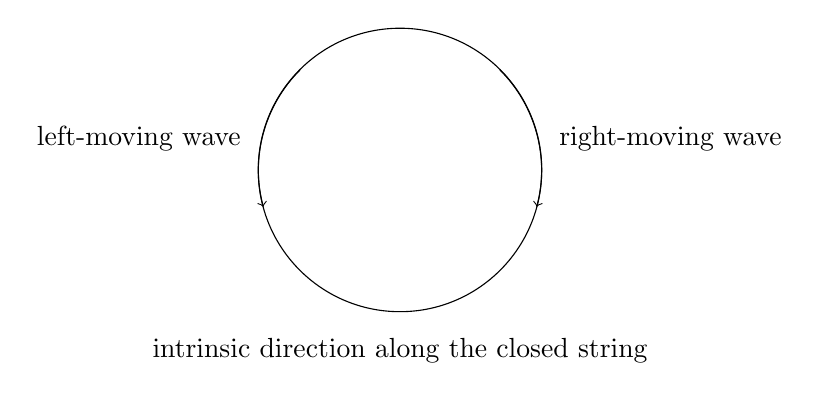
\begin{tikzpicture}[scale=1.0]
\draw (0,0) circle (1.8);
\draw[->] (1.27,1.27) arc[start angle=45,end angle=-15,radius=1.8];
\draw[->] (-1.27,1.27) arc[start angle=135,end angle=195,radius=1.8];
\node at (0,-2.3) {intrinsic direction along the closed string};
\node[right] at (1.9,0.4) {right-moving wave};
\node[left] at (-1.9,0.4) {left-moving wave};
\end{tikzpicture}
\caption{A schematic reminder that ``left'' and ``right'' refer to motion along the \(\sigma\)-coordinate, not to orientation in space.}
\end{figure}

This immediately doubles the oscillator bookkeeping. In the \(x\)-sector we have creation operators \(a_n^+\) and \(a_{-n}^+\), and in the \(y\)-sector we have \(b_n^+\) and \(b_{-n}^+\). The superscript \(+\) means creation; the sign of the subscript records the propagation direction.

\section{The First Spectrum Puzzle and the Level-Matching Rule}

At this point the lecture deliberately recalls the open-string photon. For the open string, the lowest nontrivial excitations are
\begin{equation}
a_1^+|0\rangle,
\qquad
b_1^+|0\rangle.
\end{equation}
Their circularly polarized combinations are
\begin{equation}
\big(a_1^+ \pm i b_1^+\big)|0\rangle,
\end{equation}
and these carry angular momentum \(\pm 1\) about the axis of motion.

For the closed string, if we are too quick, we would write down the four one-oscillator states
\begin{equation}
a_1^+|0\rangle,
\qquad
a_{-1}^+|0\rangle,
\qquad
b_1^+|0\rangle,
\qquad
b_{-1}^+|0\rangle.
\end{equation}
At first sight this looks like a doubled photon spectrum: two \(x\)-type and two \(y\)-type excitations, or equivalently two copies of the open-string story.

\subsection{Question \& Answer}

\paragraph{Question.} Why is this doubled-photon picture not the right closed-string spectrum?

\paragraph{Answer.} Because not every formal oscillator state is a legitimate closed-string state. There is an extra rule, introduced first as a postulate, called \emph{level matching}: the total right-moving energy must equal the total left-moving energy. Each of the states above carries excitation only in one sector or the other, so none of them survives.

Thus the one-oscillator states are ruled out. The first acceptable states occur one level higher:
\begin{equation}
a_1^+a_{-1}^+|0\rangle,
\qquad
b_1^+b_{-1}^+|0\rangle,
\qquad
a_1^+b_{-1}^+|0\rangle,
\qquad
a_{-1}^+b_1^+|0\rangle.
\end{equation}
These all carry one unit of left-moving energy and one unit of right-moving energy, so they satisfy
\begin{equation}
E_L=E_R.
\end{equation}
The lecture is explicit about the logic here: first accept level matching as a rule, then see what it does to the spectrum, and only later return to why the rule must hold.

\section{Massless Spin-2, Dilaton, and Axion}

To read off the spin content, we return to circular polarization. The four level-matched states may be reorganized as
\begin{align}
\big(a_1^+ + i b_1^+\big)\big(a_{-1}^+ + i b_{-1}^+\big)|0\rangle, \\
\big(a_1^+ - i b_1^+\big)\big(a_{-1}^+ - i b_{-1}^+\big)|0\rangle, \\
\big(a_1^+ + i b_1^+\big)\big(a_{-1}^+ - i b_{-1}^+\big)|0\rangle, \\
\big(a_1^+ - i b_1^+\big)\big(a_{-1}^+ + i b_{-1}^+\big)|0\rangle.
\end{align}
The corresponding angular momenta about the axis of motion are
\begin{align}
M &= +2, \\
M &= -2, \\
M &= 0, \\
M &= 0.
\end{align}
So the closed string does \emph{not} give a pair of photon-like states. Instead it gives one state with \(M=+2\), one with \(M=-2\), and two independent scalar states.

The crucial observation is that a \emph{massive} spin-two particle would come with five helicity states, including \(M=\pm1\) and one \(M=0\) in the appropriate basis. We do not find those. The only consistent interpretation is therefore that the \(M=\pm2\) pair forms a \emph{massless} spin-two particle. In other words, the closed string contains a graviton.

The two remaining \(M=0\) combinations are separate scalar particles. In the language of string theory they are called the dilaton and the axion. The lecture notes that both appear naturally in the closed-string spectrum, both begin massless in the formal structure, and both are far less securely tied to observed physics than the graviton itself.

\section{Why Level Matching Holds: Shifting the Origin of \(\sigma\)}

Having used level matching, the lecture returns to the deferred question. Why should the left-moving and right-moving energies be equal? The answer begins with the seemingly innocent marked point \(\sigma=0\). Is this point really special?

The discrete picture is the right place to start.

\begin{figure}[t]
\centering

\includegraphics[width=0.82\textwidth]{lecture_04_figure_03.png}
\caption{Discrete closed string and cyclic wavefunction labeling.}
\end{figure}

The board introduces the notation \(X(\sigma)\) for the continuous string and \(X_i,Y_i\) for a discretized collection of points, with \(i=1,\ldots,N\). A clean companion picture is as follows.

\begin{figure}[t]
\centering
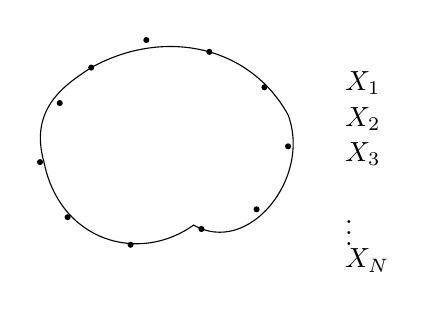
\begin{tikzpicture}[scale=1.0]
\draw
(0.2,1.0)
.. controls (1.1,1.5) and (2.2,1.3) .. (2.7,0.4)
.. controls (3.0,-0.4) and (2.2,-1.4) .. (1.5,-1.0)
.. controls (0.8,-1.5) and (-0.2,-1.2) .. (-0.4,-0.2)
.. controls (-0.6,0.5) and (-0.1,0.8) .. (0.2,1.0);
\foreach \p in {(0.2,1.0),(0.9,1.35),(1.7,1.2),(2.4,0.75),(2.7,0.0),(2.3,-0.8),(1.6,-1.05),(0.7,-1.25),(-0.1,-0.9),(-0.45,-0.2),(-0.2,0.55)}
{\fill \p circle (1.1pt);}
\node[right] at (3.3,0.8) {\(X_1\)};
\node[right] at (3.3,0.35) {\(X_2\)};
\node[right] at (3.3,-0.1) {\(X_3\)};
\node[right] at (3.3,-1.0) {\(\vdots\)};
\node[right] at (3.3,-1.45) {\(X_N\)};
\end{tikzpicture}
\caption{A discretized closed string, used to motivate cyclic relabeling.}
\end{figure}

If there is no preferred point on the loop, then the state of the string should be invariant when we relabel the points cyclically:
\begin{equation}
\Psi(x_1,x_2,\ldots,x_N)
=
\Psi(x_2,\ldots,x_N,x_1).
\end{equation}
We are not allowed to reorder the points arbitrarily; that would rip the string open. But a cyclic shift is harmless, and if the theory singled out one particular starting point it would be in real trouble.

Passing to the continuum, the discrete shift becomes
\begin{equation}
\sigma \to \sigma+\epsilon.
\end{equation}
Now the state is no longer an ordinary wave function of finitely many variables. It is a functional of the whole profile \(X(\sigma)\). The board writes this in a compressed notation, but the intended first-order statement is
\begin{equation}
0=\Psi\big(X(\sigma+\epsilon)\big)-\Psi\big(X(\sigma)\big).
\end{equation}
The close-up from the board is worth keeping, because it shows the local derivative structure very clearly.

\begin{figure}[t]
\centering

\includegraphics[width=0.72\textwidth]{lecture_04_figure_04.png}
\caption{Small-\(\epsilon\) shift of the wavefunctional argument.}
\end{figure}

At first order in \(\epsilon\), the variation is
\begin{equation}
\delta \Psi
\sim
\frac{\partial \Psi}{\partial X(\sigma)}
\frac{\partial X}{\partial \sigma}\,\epsilon.
\end{equation}
The board writes an ordinary derivative, but in the continuum it is better to interpret this as a functional derivative.

\subsection{Question \& Answer}

\paragraph{Question.} Is this a separate equation for each value of \(\sigma\)?

\paragraph{Answer.} No. That would miss the point of the symmetry. A shift of the origin of \(\sigma\) moves every point on the string at once, so the total variation is the sum over all \(\sigma\), which in the continuum becomes an integral:
\begin{equation}
\int d\sigma\,
\frac{\delta \Psi}{\delta X(\sigma)}
\,\partial_\sigma X(\sigma)=0.
\end{equation}

Now we use the standard quantum-mechanical relation between momentum and differentiation. Suppressing \(\hbar\),
\begin{equation}
P(\sigma)\sim -\,i\,\frac{\delta}{\delta X(\sigma)}.
\end{equation}
Therefore the invariance condition may be rewritten as
\begin{equation}
\int d\sigma\,P(\sigma)\,\partial_\sigma X(\sigma)=0.
\end{equation}

The board transition into this formula is also worth keeping.

\begin{figure}[t]
\centering

\includegraphics[width=0.72\textwidth]{lecture_04_figure_05.png}
\caption{Discrete shift and the emerging reparameterization constraint.}
\end{figure}

In the simple nonrelativistic string model used in the lecture, momentum is just velocity, so
\begin{equation}
P(\sigma)=\partial_\tau X(\sigma).
\end{equation}
Hence the constraint becomes
\begin{equation}
\int d\sigma\,\partial_\tau X\,\partial_\sigma X=0.
\end{equation}
This is the essential relation. Up to the same harmless normalization issues already noted in the energy split, it is precisely the difference between the left-moving and right-moving energy contributions. Thus
\begin{equation}
E_L-E_R \propto \int d\sigma\,\partial_\tau X\,\partial_\sigma X,
\end{equation}
and invariance under shifts of the \(\sigma\)-origin implies
\begin{equation}
E_L=E_R.
\end{equation}

This is the missing reason for level matching. The rule is not an arbitrary restriction placed on the spectrum from outside. It is the statement that the closed string has no physically preferred starting point.

\section{Clarifications and the Question of Fundamentality}

The lecture ends by returning once more to the language of left and right, because there are really two different uses of the words. One use refers to motion along the string, toward increasing or decreasing \(\sigma\). The other use refers to circular polarization in ordinary space, such as right-handed and left-handed photon polarization. These are not the same notion, and the distinction must be kept sharp.

Then the lecture steps back. After all these technical details of open and closed strings, one may ask whether strings are truly fundamental, or whether they might themselves be made from something else. The answer given here is deliberately cautious: ``fundamental'' is not an absolute notion. In quantum field theory one may ask whether the electron or the magnetic monopole is more fundamental, and the answer depends on which variables give a useful weakly coupled description. The same moral reappears in string theory. In one regime strings may be the natural fundamental objects; in another regime D-branes may be the simpler degrees of freedom, and strings may look composite.

That is the note on which the lecture points forward to M-theory. The real lesson is not that we have reached the end of reductionism, but that the notion of what is elementary may itself change when the parameters of the theory are changed.

\section{Summary}

We began with a brief reminder of Noether's theorem because a symmetry argument was waiting in the background. We then introduced the closed string as a loop parameterized by \(0\leq \sigma\leq 2\pi\), with one arbitrarily marked point called \(\sigma=0\), and emphasized that left- and right-moving waves refer to motion along the string rather than motion in space.

From periodic boundary conditions we obtained the Fourier expansion of the closed string and the doubling of the oscillator structure into left-moving and right-moving sectors. A naïve first guess at the spectrum gives a doubled photon-like picture, but level matching removes those states. The first surviving level-matched excitations reorganize into a massless spin-two particle, the graviton, together with two scalar states, the dilaton and the axion.

Finally, the rule \(E_L=E_R\) was derived from the statement that the closed string has no preferred point along the \(\sigma\)-circle. Cyclic relabeling in the discrete description becomes \(\sigma\to \sigma+\epsilon\) in the continuum, and invariance under that shift produces the integral constraint whose vanishing is exactly the level-matching condition. In this way the geometry of the loop, the symmetry of the \(\sigma\)-coordinate, and the structure of the spectrum are tied together.